\subsection{Thread Ring}

The thread ring benchmark originates in the Computer Language
Benchmarks Game\footnote{\url{http://shootout.alioth.debian.org/}}
(formerly known as the Great Computer Language Shootout).  It is a
simple concurrency benchmark, in which a large number of threads are
created in a ring topology, and then messages are passed around the
ring.  We include it here as an example of profiling a Concurrent
Haskell program using ThreadScope, in contrast to the other case
studies which have investigated programs that use semi-explicit
parallelism.

The code for our version of the benchmark is given in
Figure~\ref{f:threadring-code}.  This version uses a linear string of
threads rather than a ring, where a number of messages are pumped in
to the first thread in the string, and then collected at the other
end.

\begin{figure}
\begin{lstlisting}
import Control.Concurrent
import Control.Monad
import System
import GHC.Conc (forkOnIO)

thread :: MVar Int -> MVar Int -> IO ()
thread inp out = do 
  x <- takeMVar inp
  putMVar out $! x+1
  thread inp out

spawn cur n = do 
  next <- newEmptyMVar
  forkIO $ thread cur next
  return next

main = do 
  n <- getArgs >>= readIO.head
  s <- newEmptyMVar
  e <- foldM spawn s [1..2000]
  f <- newEmptyMVar
  forkIO $ replicateM n (takeMVar e) >>= putMVar f . sum
  replicateM n (putMVar s 0)
  takeMVar f
\end{lstlisting}
\caption{ThreadRing code}
\label{f:threadring-code}
\end{figure}

Our aim is to try to make this program speed up in parallel.  We
expect there to be parallelism available: multiple messages are
being pumped through the thread string, so we ought to be able to pump
messages through distinct parts of the string in parallel.

First, the sequential performance.  This is for 500 messages and 2000 threads:

\begin{verbatim}
  INIT  time    0.00s  (  0.00s elapsed)
  MUT   time    0.18s  (  0.19s elapsed)
  GC    time    0.01s  (  0.01s elapsed)
  EXIT  time    0.00s  (  0.00s elapsed)
  Total time    0.19s  (  0.21s elapsed)
\end{verbatim}

Next, running the program on two cores:

\begin{verbatim}
  INIT  time    0.00s  (  0.00s elapsed)
  MUT   time    0.65s  (  0.36s elapsed)
  GC    time    0.02s  (  0.01s elapsed)
  EXIT  time    0.00s  (  0.00s elapsed)
  Total time    0.67s  (  0.38s elapsed)
\end{verbatim}

\begin{figure*}
\begin{center}
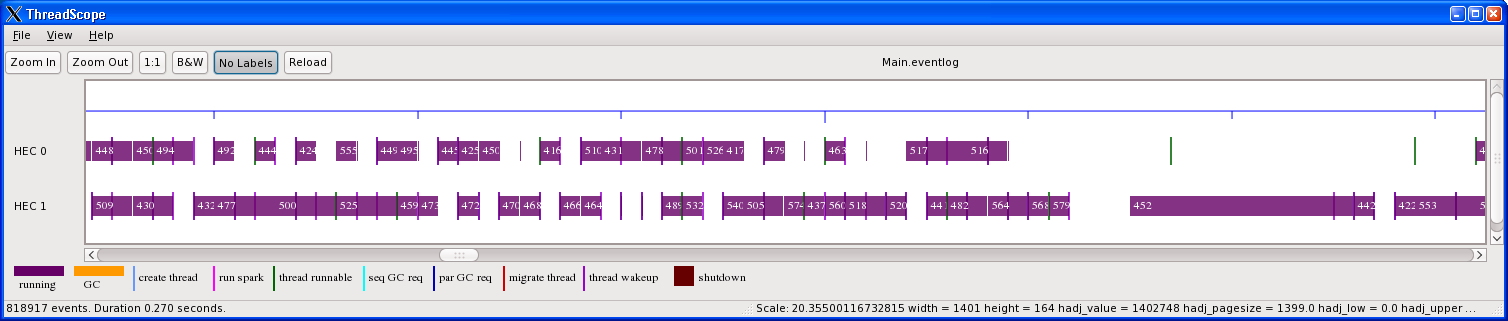
\includegraphics[scale=0.3]{threadring1.png}
\end{center}
\caption{ThreadRing profile (no explicit placement; zoomed in)}
\label{f:threadring1}
\end{figure*}

\begin{figure*}
\begin{center}
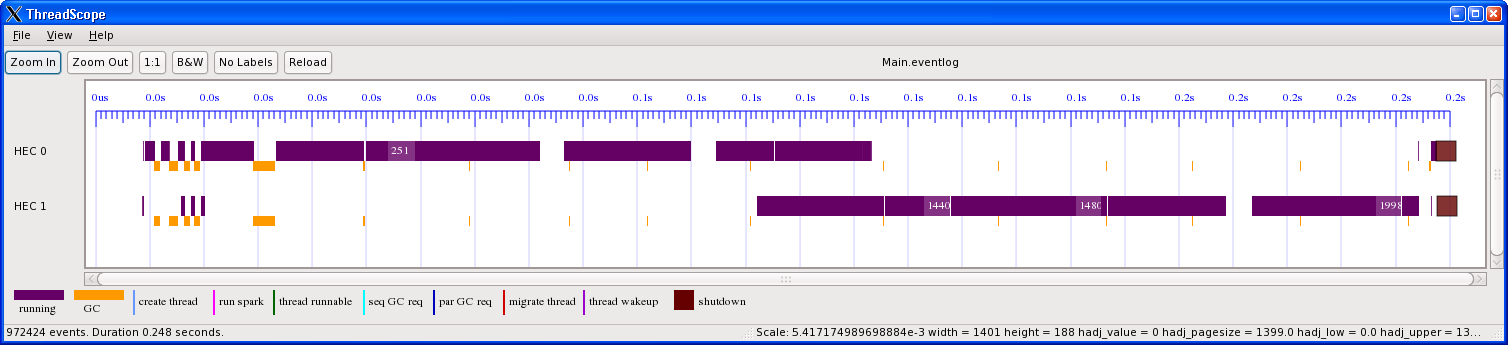
\includegraphics[scale=0.3]{threadring2.png}
\end{center}
\caption{ThreadRing profile (with explicit placement)}
\label{f:threadring2}
\end{figure*}

\begin{figure*}
\begin{center}
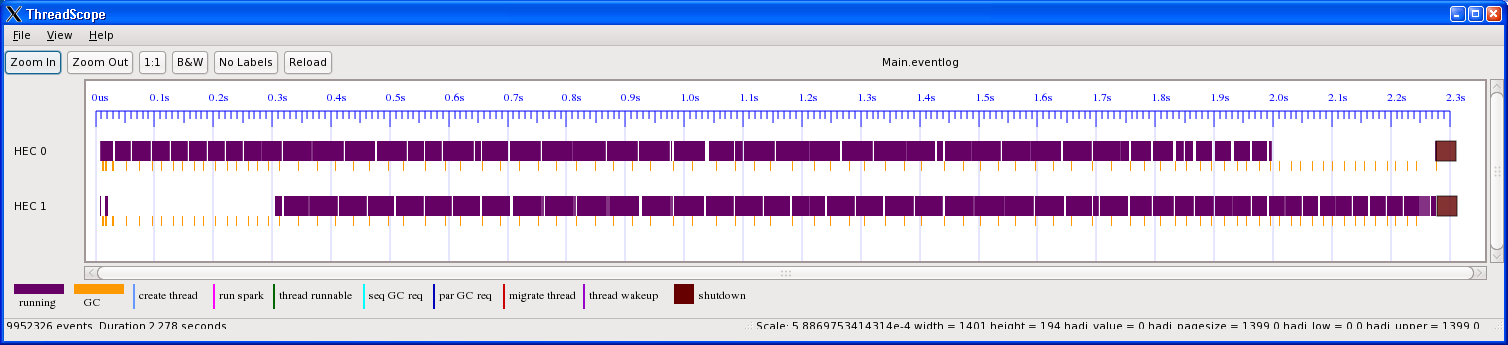
\includegraphics[scale=0.3]{threadring3.png}
\end{center}
\caption{ThreadRing profile (explicit placement and more messages)}
\label{f:threadring3}
\end{figure*}

Things are significantly slower when we add a core.  Let's examine the
ThreadScope profile to see why - at first glance, the program seems to
be using both cores, but as we zoom in we can see that there are lots
of gaps (Figure~\ref{f:threadring1}).  

In this program we want to avoid communication between the two
separate cores, because that will be expensive.  We want as much
communication as possible to happen between threads on the same core,
where it is cheap.  In order to do this, we have to give the scheduler
some help.  We know the structure of the communication in this
program: messages are passed along the string in sequence, so we can
place threads optimally to take advantage of that.  GHC provides a way
to place a thread onto a particular core (or HEC), using the
\codef{forkOnIO} operation.  The placement scheme we use is to divide
the string into linear segments, one segment per core (in our case
two).

This strategy gets us back to the same performance as the sequential
version:

\begin{verbatim}
  INIT  time    0.00s  (  0.00s elapsed)
  MUT   time    0.23s  (  0.19s elapsed)
  GC    time    0.02s  (  0.02s elapsed)
  EXIT  time    0.00s  (  0.00s elapsed)
  Total time    0.26s  (  0.21s elapsed)
\end{verbatim}

Why don't we actually see any speedup?
Figure~\ref{f:threadring2} shows the ThreadScope profile.
The program has now been almost linearized; there is a small amount of
overlap, but most of the execution is sequential, first on one core
and then the other.

Investigating the profile in more detail shows that this is a
scheduling phenomenon.  The runtime has moved all the messages through
the first string before it propagates any into the second string, and
this can happen because the total number of messages we are using for
the benchmark is less than the number of threads.  If we increase the
number of messages, then we do actually see more parallelism.
Figure~\ref{f:threadring3} shows the execution profile for 2000
messages and 2000 threads, and we can see there is significantly more
overlap.
